\subsubsection{Vaginal Births in ACT}
Vaginal birth, also known as normal vaginal delivery, is the natural way for a baby to be born through the birth canal. It offers several significant benefits for both the mother and the baby, including:

\begin{itemize}
  \item Quicker recovery: Vaginal birth typically has a shorter recovery time than a cesarean section, which is a surgical delivery. Mothers who have vaginal births can usually go home from the hospital sooner, and they often experience less pain and discomfort during the recovery period.
  \item Fewer complications: Vaginal birth is associated with fewer complications for both the mother and the baby compared to cesarean section. For example, the risk of infection, blood loss, and injury to internal organs is lower with vaginal birth.
  \item Better for breastfeeding: Babies who are born vaginally are more likely to have an easier time breastfeeding. This is because the pressure of passing through the birth canal helps to expel fluid from the baby's lungs and stimulates the release of hormones that help with breastfeeding.
  \item Improved gut health: Babies born vaginally also tend to have a healthier gut microbiome compared to those born via cesarean section. The bacteria that the baby is exposed to during vaginal birth can help to colonize the gut and support a healthy immune system.
  \item Psychological benefits: Some mothers report feeling a greater sense of empowerment and satisfaction after having a vaginal birth. This may be due to the sense of achievement and control that comes with delivering a baby without medical intervention.
\end{itemize}

Overall, vaginal birth is a safe and natural option for most women, and it offers several significant benefits for both the mother and the baby. However, it's important for each woman to discuss her individual medical history and pregnancy with her healthcare provider to determine the best course of action for her delivery.

We can see in figure \ref{fig:vaginal_act} Cesarean section method is more prominent among mothers who are over 40. Oppositely we can observe that younger women mostly have vaginal births. As the age increases the number of vaginal birth decreases and cesarean section increases.

\begin{figure}
  \centering
  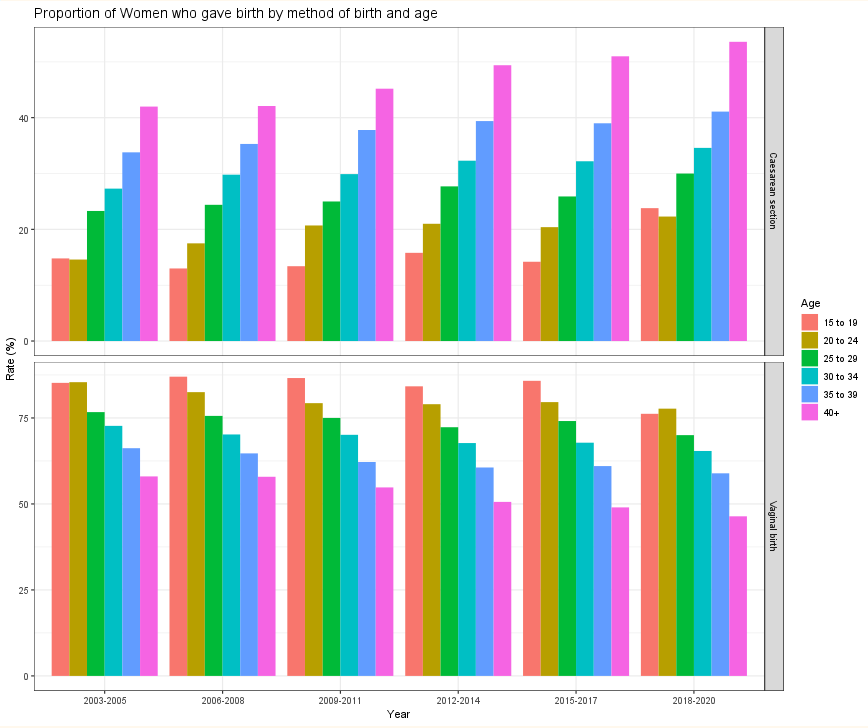
\includegraphics[width=1\textwidth]{subsections/method_of_birth/vagina_proportion.png}
  \caption{Different methods of birth in different mothers of different age groups (ACT).}
  \label{fig:vaginal_act}
\end{figure}